\section{Durchführung}

\begin{figure}[H]
  \centering
  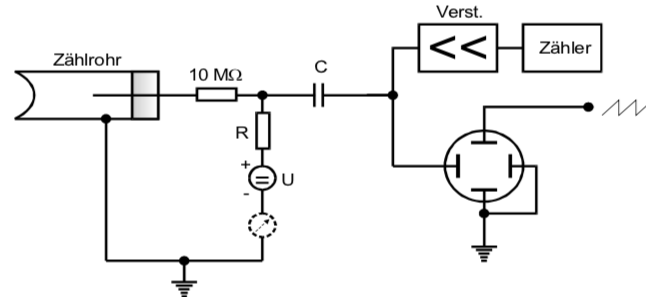
\includegraphics[width=\textwidth]{content/Aufbau.png}
  \caption{Versuchsaufbau \cite{1}.}
  \label{abb:5}
\end{figure}

In Abbildung \ref{abb:5} wird eine Skizze der Messapparatur gezeigt. Der Spannungsimpuls
wird durch den Widerstand R erzeugt und durch den Kondensator C ausgekoppelt. Daraufhin
wird der Impuls noch verstärkt und die Impulse können duch ein Zählgerät oder Oszilloskop
aufgezeichnet werden. Für alle Messreihen ist $\Delta t = \SI{60}{\second}$.

Als erstes wird die Charakteristik des Zählrohrs betrachtet. Dazu wird die Zählrate
in Abhängigkeit der Spannung gemessen. Es wird von \SI{300}{\volt} bis \SI{700}{\volt} gemessen.
Parallel dazu wird auch der Strom gemessen. Mit der folgenden Gleichung kann aus
dem gemessenen Strom auf die Ladungsmenge geschlossen werden.

\begin{equation}
  \overline{I} = \frac{\Delta Q}{\Delta t} Z
  \label{eq:1}
\end{equation}

Dabei sind Z die Teilchen die pro Zeit $\Delta t$ gemessen werden.

Daraufhin wird für drei verschiedene Spannungen die Totzeit untersucht. Dafür
werden die Messwerte auf einem Oszilloskop aufgetragen und erhalten ein Bild wie
in Abbildung \ref{abb:3}. Von dem Oszilloskop werden dann die Totzeit und Erholungszeit
abgelesen.

Als letzte wird die Totzeit durch die Zwei-Quellen-Methode bestimmt. Dazu wird zunächst
die Zählrate von Präparat 1 bestimmt, danach von Präparat 1 und 2 zusammen und als letztes
die von Präparat 2. Aufgrund der Totzeit wird $N_{1+2} < N_1 + N_2$ und mit der
Gleichung \ref{eq:2} lässt sich die Totzeit berechnen.

\begin{equation}
  T \approx \frac{N_1 + N_2 - N_{1+2}}{2 N_1 N_2}
  \label{eq:2}
\end{equation}





Da die Darstellung der Messdaten nicht auf die Seite passen werden sie in zwei Teile aufgeteilt.
\begin{table}[H]
  \centering
  \caption{Messung bei $U=520 \, V$ und $\Delta t = 60 \, s$(Teil 1).}
  \label{tab:3}
      \begin{tabular}{c c c c c c}
        \toprule
        $U \, /\, V$ & $I \,/\, \mu A $ & $n \,/\, 10^{10} Teilchen$ &
        $U \, /\, V$ & $I \,/\, \mu A $ & $n \,/\, 10^{10} Teilchen$ &
        $U \, /\, V$ & $I \,/\, \mu A $ & $n \,/\, 10^{10} Teilchen$ &
        $U \, /\, V$ & $I \,/\, \mu A $ & $n \,/\, 10^{10} Teilchen$ \\
        \midrule
        340 & 0.2 & 0.599 \pm 0.005 & 440 & 0.4 & 1.138 \pm 0.009 \\
        350 & 0.2 & 0.588 \pm 0.005 & 450 & 0.5 & 1.421 \pm 0.012 \\
        360 & 0.2 & 0.584 \pm 0.005 & 460 & 0.5 & 1.424 \pm 0.012 \\
        310 & 0.1 & 0.309 \pm 0.002 & 410 & 0.3 & 0.855 \pm 0.007 \\
        320 & 0.2 & 0.596 \pm 0.005 & 420 & 0.4 & 1.146 \pm 0.010 \\
        330 & 0.2 & 0.591 \pm 0.005 & 430 & 0.4 & 1.158 \pm 0.010 \\
        370 & 0.2 & 0.579 \pm 0.005 & 470 & 0.5 & 1.441 \pm 0.013 \\
        380 & 0.3 & 0.869 \pm 0.007 & 480 & 0.6 & 1.704 \pm 0.015 \\
        390 & 0.3 & 0.879 \pm 0.008 & 490 & 0.6 & 1.728 \pm 0.015 \\
        400 & 0.3 & 0.860 \pm 0.008 & 500 & 0.6 & 1.691 \pm 0.014 \\
        \bottomrule
      \end{tabular}
    \end{table}

    \begin{table}[H]
      \centering
      \caption{Messung bei $U=520 \, V$ und $\Delta t = 60 \, s$ (Teil 2).}
      \label{tab:4}
          \begin{tabular}{c c c c c c}
            \toprule
            $U \, /\, V$ & $I \,/\, \mu A $ & $n \,/\, 10^{10} Teilchen$ &
            $U \, /\, V$ & $I \,/\, \mu A $ & $n \,/\, 10^{10} Teilchen$ &\\
            \midrule
            510 & 0.6 & 1.721 \pm 0.015 & 610 & 0.9 & 2.539 \pm 0.022\\
            520 & 0.6 & 1.684 \pm 0.015 & 620 & 1.0 & 2.789 \pm 0.023\\
            530 & 0.7 & 1.968 \pm 0.017 & 630 & 1.0 & 2.779 \pm 0.024\\
            540 & 0.7 & 1.985 \pm 0.017 & 640 & 1.0 & 2.765 \pm 0.024\\
            550 & 0.8 & 2.253 \pm 0.020 & 650 & 1.0 & 2.695 \pm 0.023\\
            560 & 0.8 & 2.243 \pm 0.019 & 660 & 1.0 & 2.735 \pm 0.023\\
            570 & 0.8 & 2.273 \pm 0.020 & 670 & 1.1 & 3.006 \pm 0.026\\
            580 & 0.8 & 2.219 \pm 0.019 & 680 & 1.1 & 2.964 \pm 0.025\\
            590 & 0.8 & 2.232 \pm 0.019 & 690 & 1.2 & 3.294 \pm 0.028\\
            600 & 0.9 & 2.526 \pm 0.022 & 700 & 1.3 & 3.409 \pm 0.029\\
            \bottomrule
          \end{tabular}
        \end{table}
